% hw5.tex

% !TEX program = xelatex
%%%%%%%%%%%%%%%%%%%%
% see http://mirrors.concertpass.com/tex-archive/macros/latex/contrib/tufte-latex/sample-handout.pdf
% for how to use tufte-handout
\documentclass[a4paper, justified]{tufte-handout}

% hw-preamble.tex

% geometry for A4 paper
% See https://tex.stackexchange.com/a/119912/23098
\geometry{
  left=20.0mm,
  top=20.0mm,
  bottom=20.0mm,
  textwidth=130mm, % main text block
  marginparsep=5.0mm, % gutter between main text block and margin notes
  marginparwidth=50.0mm % width of margin notes
}

% for colors
\usepackage{xcolor} % usage: \color{red}{text}
% predefined colors
\newcommand{\red}[1]{\textcolor{red}{#1}} % usage: \red{text}
\newcommand{\blue}[1]{\textcolor{blue}{#1}}
\newcommand{\teal}[1]{\textcolor{teal}{#1}}

\usepackage{todonotes}

% heading
\usepackage{sectsty}
\setcounter{secnumdepth}{2}
\allsectionsfont{\centering\huge\rmfamily}

% for Chinese
\usepackage{xeCJK}
\usepackage{zhnumber}
\setCJKmainfont[BoldFont=FandolSong-Bold.otf]{FandolSong-Regular.otf}

% for fonts
\usepackage{fontspec}
\newcommand{\song}{\CJKfamily{song}}
\newcommand{\kai}{\CJKfamily{kai}}

% To fix the ``MakeTextLowerCase'' bug:
% See https://github.com/Tufte-LaTeX/tufte-latex/issues/64#issuecomment-78572017
% Set up the spacing using fontspec features
\renewcommand\allcapsspacing[1]{{\addfontfeature{LetterSpace=15}#1}}
\renewcommand\smallcapsspacing[1]{{\addfontfeature{LetterSpace=10}#1}}

% for url
\usepackage{hyperref}
\hypersetup{colorlinks = true,
  linkcolor = teal,
  urlcolor  = teal,
  citecolor = blue,
  anchorcolor = blue}

\newcommand{\me}[4]{
    \author{
      {\bfseries 姓名:}\underline{#1}\hspace{2em}
      {\bfseries 学号:}\underline{#2}\hspace{2em}\\[10pt]
      {\bfseries 评分:}\underline{#3\hspace{3em}}\hspace{2em}
      {\bfseries 评阅:}\underline{#4\hspace{3em}}
  }
}

% Please ALWAYS Keep This.
\newcommand{\noplagiarism}{
  \begin{center}
    \fbox{\begin{tabular}{@{}c@{}}
      请独立完成作业,不得抄袭。\\
      若得到他人帮助, 请致谢。\\
      若参考了其它资料,请给出引用。\\
      鼓励讨论,但需独立书写解题过程。
    \end{tabular}}
  \end{center}
}

% \newcommand{\goal}[1]{
%   \begin{center}{\fcolorbox{blue}{yellow!60}{\parbox{0.50\textwidth}{\large
%     \begin{itemize}
%       \item 体会``思维的乐趣''
%       \item 初步了解递归与数学归纳法
%       \item 初步接触算法概念与问题下界概念
%     \end{itemize}}}}
%   \end{center}
% }

% Each hw consists of four parts:
\newcommand{\beginrequired}{\hspace{5em}\section{作业 (必做部分)}}
\newcommand{\beginoptional}{\section{作业 (选做部分)}}
\newcommand{\beginot}{\section{Open Topics}}
\newcommand{\begincorrection}{\section{订正}}
\newcommand{\beginfb}{\section{反馈}}

% for math
\usepackage{amsmath, mathtools, amsfonts, amssymb}
\newcommand{\set}[1]{\{#1\}}

% define theorem-like environments
\usepackage[amsmath, thmmarks]{ntheorem}

\theoremstyle{break}
\theorempreskip{2.0\topsep}
\theorembodyfont{\song}
\theoremseparator{}
\newtheorem{problem}{题目}[subsection]
\renewcommand{\theproblem}{\arabic{problem}}
\newtheorem{ot}{Open Topics}

\theorempreskip{3.0\topsep}
\theoremheaderfont{\kai\bfseries}
\theoremseparator{:}
\theorempostwork{\bigskip\hrule}
\newtheorem*{solution}{解答}
\theorempostwork{\bigskip\hrule}
\newtheorem*{revision}{订正}

\theoremstyle{plain}
\newtheorem*{cause}{错因分析}
\newtheorem*{remark}{注}

\theoremstyle{break}
\theorempostwork{\bigskip\hrule}
\theoremsymbol{\ensuremath{\Box}}
\newtheorem*{proof}{证明}

% \newcommand{\ot}{\blue{\bf [OT]}}

% for figs
\renewcommand\figurename{图}
\renewcommand\tablename{表}

% for fig without caption: #1: width/size; #2: fig file
\newcommand{\fig}[2]{
  \begin{figure}[htbp]
    \centering
    \includegraphics[#1]{#2}
  \end{figure}
}
% for fig with caption: #1: width/size; #2: fig file; #3: caption
\newcommand{\figcap}[3]{
  \begin{figure}[htbp]
    \centering
    \includegraphics[#1]{#2}
    \caption{#3}
  \end{figure}
}
% for fig with both caption and label: #1: width/size; #2: fig file; #3: caption; #4: label
\newcommand{\figcaplbl}[4]{
  \begin{figure}[htbp]
    \centering
    \includegraphics[#1]{#2}
    \caption{#3}
    \label{#4}
  \end{figure}
}
% for margin fig without caption: #1: width/size; #2: fig file
\newcommand{\mfig}[2]{
  \begin{marginfigure}
    \centering
    \includegraphics[#1]{#2}
  \end{marginfigure}
}
% for margin fig with caption: #1: width/size; #2: fig file; #3: caption
\newcommand{\mfigcap}[3]{
  \begin{marginfigure}
    \centering
    \includegraphics[#1]{#2}
    \caption{#3}
  \end{marginfigure}
}

\usepackage{fancyvrb}

% for algorithms
\usepackage[]{algorithm}
\usepackage[]{algpseudocode} % noend
% See [Adjust the indentation whithin the algorithmicx-package when a line is broken](https://tex.stackexchange.com/a/68540/23098)
\newcommand{\algparbox}[1]{\parbox[t]{\dimexpr\linewidth-\algorithmicindent}{#1\strut}}
\newcommand{\hStatex}[0]{\vspace{5pt}}
\makeatletter
\newlength{\trianglerightwidth}
\settowidth{\trianglerightwidth}{$\triangleright$~}
\algnewcommand{\LineComment}[1]{\Statex \hskip\ALG@thistlm \(\triangleright\) #1}
\algnewcommand{\LineCommentCont}[1]{\Statex \hskip\ALG@thistlm%
  \parbox[t]{\dimexpr\linewidth-\ALG@thistlm}{\hangindent=\trianglerightwidth \hangafter=1 \strut$\triangleright$ #1\strut}}
\makeatother

% for footnote/marginnote
% see https://tex.stackexchange.com/a/133265/23098
\usepackage{tikz}
\newcommand{\circled}[1]{%
  \tikz[baseline=(char.base)]
  \node [draw, circle, inner sep = 0.5pt, font = \tiny, minimum size = 8pt] (char) {#1};
}
\renewcommand\thefootnote{\protect\circled{\arabic{footnote}}}

\newcommand{\score}[1]{{\bf [#1 分]}}

\newcommand{\rel}[1]{\xrightarrow{#1}}
\newcommand{\dstar}{\xRightarrow[]{\ast}}
\newcommand{\dplus}{\xRightarrow[]{+}}
\newcommand{\lm}{\xRightarrow[\text{lm}]{}}
\renewcommand{\rm}{\xRightarrow[\text{rm}]{}}
\newcommand{\dpluslm}{\xRightarrow[\text{lm}]{+}}
\newcommand{\dstarlm}{\xRightarrow[\text{lm}]{\ast}}
\newcommand{\dplusrm}{\xRightarrow[\text{rm}]{+}}
\newcommand{\dstarrm}{\xRightarrow[\text{rm}]{\ast}}

\newcommand{\sep}{\;\big\lvert\;}

\newcommand{\first}{\textsc{First}}
\newcommand{\follow}{\textsc{Follow}}

% see https://tex.stackexchange.com/a/109906/23098
\usepackage{empheq}
\newcommand*\widefbox[1]{\fbox{\hspace{2em}#1\hspace{2em}}} % feel free to modify this file if you understand LaTeX well
\usetikzlibrary{shapes.multipart,arrows,automata,positioning}
\usepackage{multirow}
%%%%%%%%%%%%%%%%%%%%
\title{编译原理作业 (5)}
\me{王腾}{171240540@smial.nju.edu.cn}{}{}
\date{\today}
%%%%%%%%%%%%%%%%%%%%
\begin{document}
\maketitle
%%%%%%%%%%%%%%%%%%%%
\noplagiarism % PLEASE DON'T DELETE THIS LINE!
%%%%%%%%%%%%%%%%%%%%
\begin{abstract}
  % \mfigcap{width = 0.85\textwidth}{figs/George-Boole}{George Boole}
  % \begin{center}{\fcolorbox{blue}{yellow!60}{\parbox{0.65\textwidth}{\large
  %   \begin{itemize}
  %     \item
  %   \end{itemize}}}}
  % \end{center}
\end{abstract}
%%%%%%%%%%%%%%%%%%%%
\beginrequired
%%%%%%%%%%%%%%%

%%%%%%%%%%%%%%%
\begin{problem}[\score{10 = 1 + 4 + 2 + 3}]
  给定下述文法$G$,
  \begin{align}
    L &\to LP \\[8pt]
    L &\to P \\[8pt]
    P &\to (P) \\[8pt]
    P &\to ()
  \end{align}

  \begin{enumerate}[(1)]
    \item 为后面的小题计算必要的\first{}集合与\follow{}集合 (可以直接转抄上次作业);
    \item 为 $G$ 构造 $LR(1)$ 自动机;

      注意: 为了尽量统一状态编号, 便于批改, 当计算\textsc{closure}时, 请按照文法编号大小顺序加入新项。
      当计算\textsc{goto}$(I, X)$时, 请按照$I$中项的出现顺序依次考虑可能的转移符号$X$。
      
      要求: 给出初始状态$I_{0}$的计算方法以及\textsc{goto}($I_{0}, ($)的计算方法。
    \item 为该文法设计$LR(1)$分析表; 该文法是$LR(1)$文法吗? 请说明理由。

      要求: 请说明归约的设置条件。
    \item 为该文法设计$LALR(1)$分析表; 该文法是$LALR(1)$文法吗? 请说明理由。
  \end{enumerate}
\end{problem}

\begin{solution}
\begin{enumerate}[(1)]
    \item \first{(L)}=\{(\}, \follow{(L)}=\{$\$,($\},\first{(P)}=\{$($\},\follow{(P)}=\{$\$,(,)$\}
    \item  
    \begin{itemize}
        \item[*] 增加产生式$L'\to L$,$I_0=$\textsc{closure}(\{$[L'\to \cdot L,\$]$\})
        \item[1] $[L'\to \cdot L,\$]$产生项:$[L\to \cdot LP,\$]$, $[L\to \cdot P,\$]$
        \item[2] $[L\to \cdot LP,\$]$产生项:$[L\to \cdot LP,(]$, $[L\to \cdot P,(]$
        \item[2] $[L\to \cdot P,\$]$产生项:$[P\to \cdot (P),\$]$, $[P\to \cdot (),\$]$
        \item[3] $[L\to \cdot P,(]$产生项:$[P\to \cdot (P),(]$, $[P\to \cdot (),(]$
        \item $I_0$=\Big\{ $[L'\to \cdot L,\$], [L\to \cdot LP,\{\$,(\}],[L\to \cdot P,\{\$,(\}],[P\to \cdot (P),\{\$,(\}],$ \\$[P\to \cdot (),\{\$,(\}]$\Big\}
        \item \textsc{goto}($I_0,($)=\textsc{closure}(\big\{ $[P\to (\cdot P),\{\$,(\}], [P\to (\cdot),\{\$,(\}]$ \big\})
        \item[*] LR(1)自动机:\\
        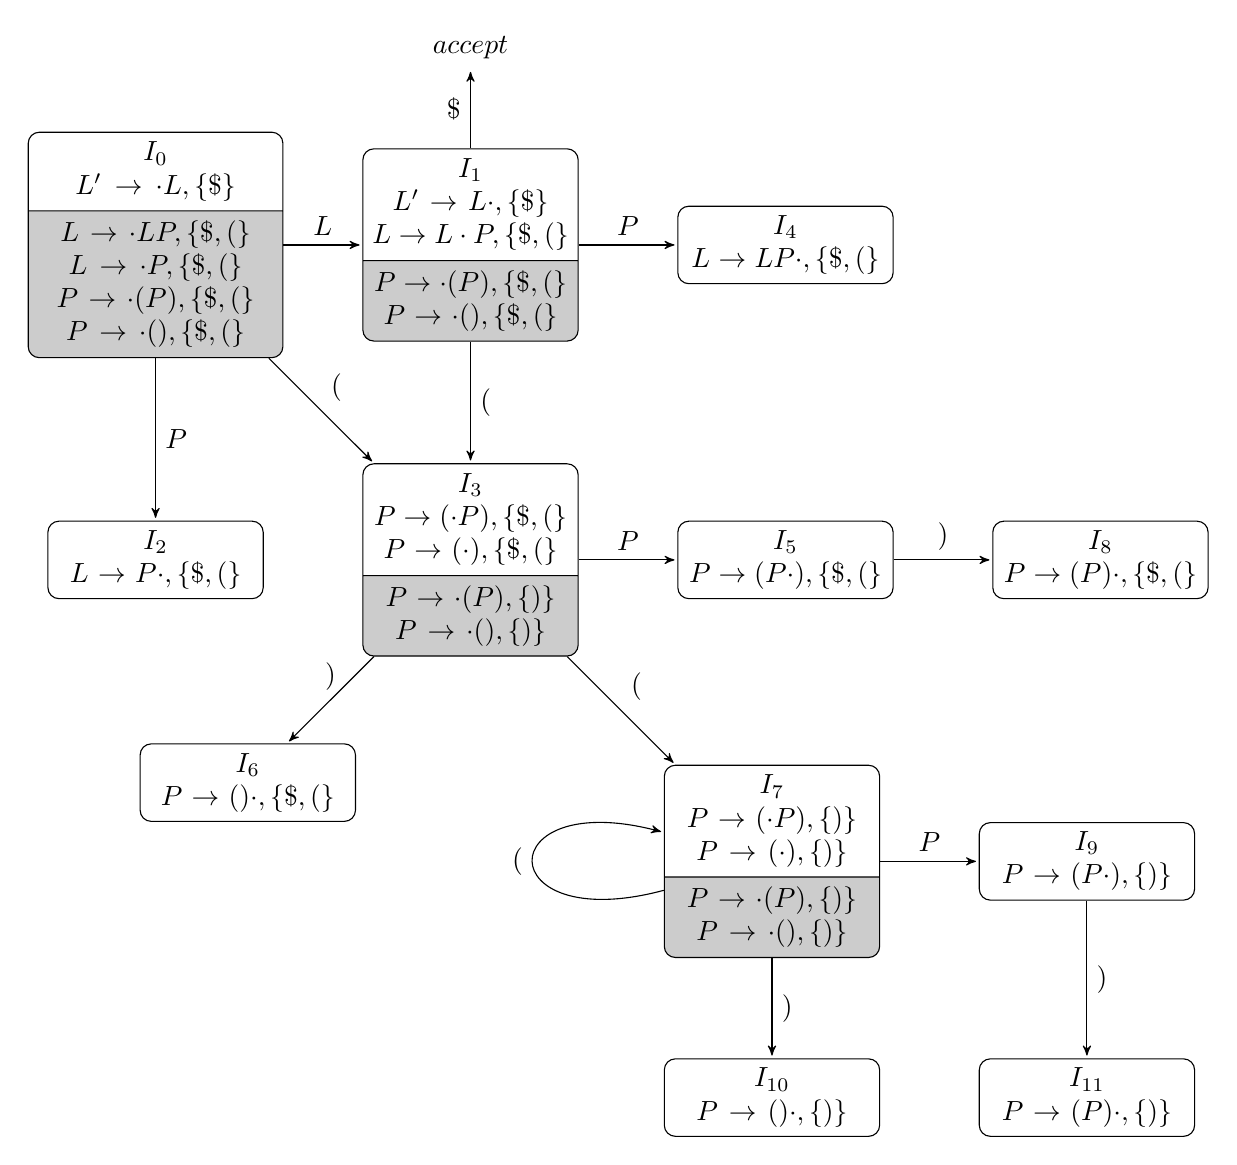
\begin{tikzpicture}[->,>=stealth',shorten >=1pt,node distance=4cm,on grid,scale = 1, auto]
            
            \node (0) [ draw,rounded corners, text centered, text width=3cm, rectangle split, rectangle split parts=2,rectangle split part fill={white,gray!40}]
                {
                    $I_0$\\
                    $L'\to \cdot L,\{\$\}$
                    \nodepart{two}
                    $L\to \cdot LP,\{\$,(\}$\\
                    $L\to \cdot P,\{\$,(\}$\\
                    $P\to \cdot (P),\{\$,(\}$\\
                    $P\to \cdot (),\{\$,(\}$
                };
            \node (1) [right of=0,draw,rounded corners, text centered, text width=2.5cm, rectangle split, rectangle split parts=2,rectangle split part fill={white,gray!40}]
            {
                $I_1$\\
                $L'\to L\cdot,\{\$\}$\\
                $L\to L\cdot P,\{\$,(\}$
                \nodepart{two}
                $P\to \cdot (P),\{\$,(\}$\\
                $P\to \cdot (),\{\$,(\}$
            };
            \node (2) [below of=0,draw,rounded corners, text centered, text width=2.5cm]
            {
                $I_2$\\
                $L\to P\cdot,\{\$,(\} $
            };
            \node (3) [below of=1,draw,rounded corners, text centered, text width=2.5cm, rectangle split, rectangle split parts=2,rectangle split part fill={white,gray!40}]
            {
                $I_3$\\
                $P\to (\cdot P),\{\$,(\} $\\
                $P\to (\cdot ),\{\$,(\}$
                \nodepart{two}
                $P\to \cdot (P),\{)\}$\\
                $P\to \cdot (),\{)\}$
            };
            \node (4) [right of=1,draw,rounded corners, text centered, text width=2.5cm]
            {
                $I_4$\\
                $L\to LP\cdot,\{\$,(\} $
            };
            \node (5) [right of=3,draw,rounded corners, text centered, text width=2.5cm]
            {
                $I_5$\\
                $P\to (P\cdot),\{\$,(\} $
            };
            \node (6) [below left of=3,draw,rounded corners, text centered, text width=2.5cm]
            {
                $I_6$\\
                $P\to ()\cdot,\{\$,(\} $
            };
            \node (7) [below right of=3,xshift=1cm,yshift=-1cm, draw,rounded corners, text centered, text width=2.5cm, rectangle split, rectangle split parts=2,rectangle split part fill={white,gray!40}]
            {
                $I_7$\\
                $P\to (\cdot P),\{)\} $\\
                $P\to (\cdot ),\{)\}$
                \nodepart{two}
                $P\to \cdot (P),\{)\}$\\
                $P\to \cdot (),\{)\}$
            };
            \node (8) [right of=5,draw,rounded corners, text centered, text width=2.5cm]
            {
                $I_8$\\
                $P\to (P)\cdot,\{\$,(\} $
            };
            \node (9) [right of=7,draw,rounded corners, text centered, text width=2.5cm]
            {
                $I_9$\\
                $P\to (P\cdot),\{)\} $
            };
            \node (10) [below of=7,yshift=1cm,draw,rounded corners, text centered, text width=2.5cm]
            {
                $I_{10}$\\
                $P\to ()\cdot,\{)\} $
            };
            \node (11) [below of=9,yshift=1cm,draw,rounded corners, text centered, text width=2.5cm]
            {
                $I_{11}$\\
                $P\to (P)\cdot,\{)\} $
            };
            \node (12) [above of=1,yshift=-1.5cm] {$accept$};

            \path 
                    (0) edge              node {$L$} (1)
                    (0) edge              node {$P$} (2)
                    (0) edge              node {$($} (3)
                    (1) edge              node {$P$} (4)
                    (1) edge              node {$($} (3)
                    (1) edge              node {$\$$} (12)
                    (3) edge              node {$P$} (5)
                    (3) edge[above]       node {$)$} (6)
                    (3) edge              node {$($} (7)
                    (5) edge              node {$)$} (8)
                    (7) edge[loop left]   node {$($} (7)
                    (7) edge              node {$P$} (9)
                    (7) edge              node {$)$} (10)
                    (9) edge              node {$)$} (11);

        \end{tikzpicture}
    \end{itemize}
    \item 按$X\to \gamma$, \textsc{sym}规约时,当前分析的非终结符号$a$要满足:$a\in$ \textsc{sym}\\
    \begin{tabular}{|c|c|c|c|c|c|}
        \hline
                                                   & \multicolumn{3}{c|}{ACTION} & \multicolumn{2}{c|}{GOTO} \\ \hline 
                                                   & (       & )       & \$       & L           & P           \\ \hline
        0                                          & s3      &         &         & g1          & g2          \\ \hline
        1                                          & s3      &         & accept     &             & g4          \\ \hline
        2                                          & r2      &         & r2      &             &             \\ \hline
        3                                          & s7      & s6      &         &             & g5          \\ \hline
        4                                          & r1      &         & r1      &             &             \\ \hline
        5                                          &         & s8      &         &             &             \\ \hline
        6                                          & r4      &         & r4      &             &             \\ \hline
        7                                          & s7      & s10     &         &             & g9          \\ \hline
        8                                          & r3      &         & r3      &             &             \\ \hline
        9                                          &         & s11     &         &             &             \\ \hline
        10                                         &         & r4      &         &             &             \\ \hline
        11                                         &         & r3      &         &             &             \\ \hline
        \end{tabular}\\
        该文法是$LR(1)$文法,因为$LR(1)$预测分析表没有冲突
    \item LALR(1)预测分析表:\\
    \begin{tabular}{|c|c|c|c|c|c|}
        \hline
            & \multicolumn{3}{c|}{ACTION} & \multicolumn{2}{c|}{GOTO} \\ \hline
            & (      & )       & \$        & L           & P           \\ \hline
        0   & s37    &         &          & g1          & g2          \\ \hline
        1   & s37     &         & accept   &             & g4          \\ \hline
        2   & r2     &         & r2       &             &             \\ \hline
        37  & s37    & s610    &          &             & g59         \\ \hline
        4   & r1     &         & r1       &             &             \\ \hline
        59  &        & s811    &          &             &             \\ \hline
        610 & r4     & r4      & r4       &             &             \\ \hline
        811 & r3     & r3      & r3       &             &             \\ \hline
        \end{tabular}\\
        该文法是LALR(1)文法,因为LALR(1)预测分析表无冲突
\end{enumerate}
\end{solution}
%%%%%%%%%%%%%%%

%%%%%%%%%%%%%%%%%%%%
% 如果没有需要订正的题目,可以把这部分删掉

% \begincorrection
%%%%%%%%%%%%%%%%%%%%

%%%%%%%%%%%%%%%%%%%%
% 如果没有反馈,可以把这部分删掉

%%%%%%%%%%%%%%%%%%%%
\end{document}